% \documentclass[handout]{beamer}
\documentclass[presentation]{beamer}

\usepackage[utf8]{inputenc}
\usepackage[UKenglish]{babel}
\usepackage[T1]{fontenc}
\usepackage{lmodern}
\usepackage{booktabs}
\usepackage{caption}
\usepackage{subcaption}
\usepackage{graphicx}
\usepackage{amsmath}
\usepackage{amsfonts}
\usepackage{amssymb}
\usepackage{epstopdf}
\usepackage{hyperref}

\usepackage[backend=bibtex, sorting=ydnt, style=numeric-comp, defernumbers]{biblatex}
\addbibresource{references.bib}

\usepackage{tikz}
\usetikzlibrary{positioning,calc}
%\usetikzlibrary{external}
%\tikzexternalize[prefix=fig/]

% complying UK date format, i.e. 1 January 2001
\usepackage{datetime}
\let\dateUKenglish\relax
\newdateformat{dateUKenglish}{\THEDAY~\monthname[\THEMONTH] \THEYEAR}

\usecolortheme{Imperial}
% 
\newcommand{\NN}{{\mathcal{N}}}
\newcommand{\mean}[1]{\mathbf{E}\left[#1\right]}
\newcommand{\inv}[1]{{#1}^{-1}}
\DeclareMathOperator{\rank}{\mathrm{rank}}
\DeclareMathOperator{\cov}{\mathrm{Cov}}
\DeclareMathOperator{\var}{\mathrm{Var}}
\newcommand{\col}[1]{\underset{{#1}}{\mathrm{col}}}
\newcommand{\row}[1]{\underset{{#1}}{\mathrm{row}}}
\newcommand{\diag}[1]{\underset{{#1}}{\textrm{diag}}}

%------------------------------------------------------------------------
%Information to be included in the title page:
\title{Addressing Security in Control Systems}
\subtitle{Overview and Current Directions}
\author{Angelo Barboni}

\date{17 September 2019}

\begin{document}
 
\begin{frame}[noframenumbering,plain]
\titlepage
\end{frame}

\begin{frame}[noframenumbering,plain]{Outline}
    \tableofcontents
\end{frame}


\section{Introduction}

\begin{frame}
	\frametitle{Security goals}

	Security (of information) can be attained if these properties are satisfied:
	\vfill
	\begin{description}
		\item[Confidentiality] Concealment or protection of sensitive information
		\item[Integrity] Trustworthiness and authenticity of data or resources 
		\item[Availability] Reliable and timely access to desired information 
	\end{description}
	\vfill
	\null
\end{frame}

\begin{frame}
	\frametitle{Motivation}
	\begin{center}
		Cyber-Physical Systems (CPS) $=$ \\ (complex, connected) software $+$ hardware
	\end{center}
	\vspace{-1ex}
	\begin{columns}
		\begin{column}{0.35\textwidth}
			Software is vulnerable: it \emph{will} be exploited. 

			\vspace{3ex}
			Security has be thought of in a system way.
		\end{column}
		\begin{column}{0.64\textwidth}
			\begin{figure}
				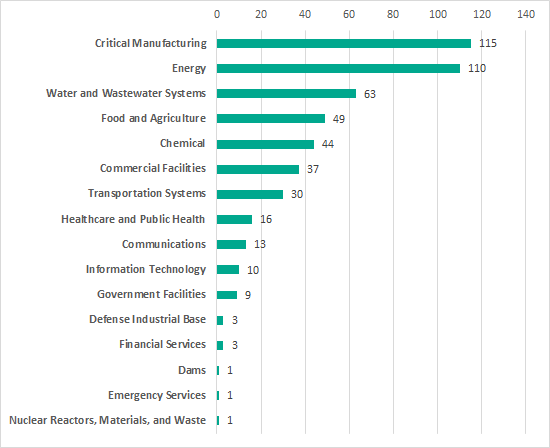
\includegraphics[scale=0.44]{fig/vuln-report-ics-cert.png}
				\caption*{\scriptsize Vulnerabilities in 2018 by sector [\href{https://ics-cert.us-cert.gov/}{\color{blue}{\underline{US ICS-CERT}}}]}
			\end{figure}
		\end{column}
	\end{columns}
\end{frame}

\begin{frame}
	\frametitle{A (possibly incomplete) series of unfortunate events}
	\setbeamertemplate{description item}[align left]
	\begin{description}
		\item[2000] Maroochy Shire incident (Australia)
		\item[2007] Aurora generator test (USA)
		\item[2009-2010] Stuxnet worm (Iran)
		\item[2014] Steel mill (Germany)
		\item[2015] Blackout (Ukraine)
		\item[2017] TRITON malware, oil spill (Saudi Arabia)
		\item[2019] Power grid DoS (USA)  
	\end{description}
\end{frame}

\begin{frame}
	\frametitle{Disclaimer}

	The topic of security encompasses many fields, from dedicated software security (PLCs, SCADA systems), to application specific cases (power networks, mobile networks, multiagent systems, etc.).

	\vfill
	We follow a generic system (model-based) approach.
\end{frame}

\AtBeginSection[]
{
	\begin{frame}[noframenumbering,plain]{Outline}
		\tableofcontents[currentsection, hideallsubsections]
	\end{frame}
}

\section{Modelling}

\begin{frame}
	\frametitle{System model}
	We consider dynamical systems in the form 

	\begin{align*}
		%\label{eq:dynsys}
		\mathcal P: \left\lbrace
		\begin{aligned}
			&\dot x = f(t,x,\textcolor{red}{\tilde u},w) \\
			&y = h(t,x,\textcolor{red}{\tilde u},v),
		\end{aligned}\right.
	\end{align*}

	but typically linearity is assumed 

	\begin{align*}
	%\label{eq:ltiplant}
	\mathcal P : \left\lbrace
	\begin{aligned}
		&\dot x = Ax + B\textcolor{red}{\tilde u} + Ww\\
		&y = Cx + D\textcolor{red}{\tilde u} + Vv
	\end{aligned}\right.
	\end{align*}
\end{frame}

\begin{frame}
	\frametitle{Adversarial model}
	An attack can be described as a triplet $\{\mathcal K, \mathcal R, g\}$ of
	\smallskip
	\begin{itemize}
		\item<1-> Knowledge $\mathcal K$ on the system, i.e. system matrices, type of detector used, etc.
		\item<2-> Resources $\mathcal R$, i.e. the measurement and actuation signals that can be accessed and/or altered
		\item<3> Attack strategy $g$ that describes the (unknown) attack strategy as some function of the available information.
	\end{itemize}	
\end{frame}

\begin{frame}
	\frametitle{Adversarial model (cont'd)}
	\begin{columns}
		\begin{column}{0.49\textwidth}
			\resizebox{\textwidth}{!}{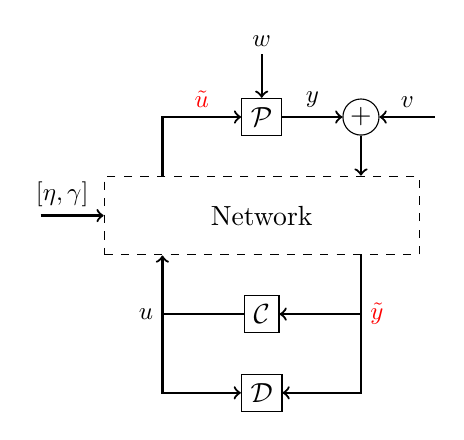
\begin{tikzpicture}{node distance=.5cm,semithick}

\node[draw] (plant) at (0,0) {$\mathcal{P}$};
\node[
   draw,
   dashed,
   minimum width = 4cm,
   minimum height = 1cm,
   below = .5cm of plant 
] (network) {Network};
\node[draw, below = .5cm of network] (controller) {$\mathcal{C}$}; 
\node[draw, below of = controller] (detector) {$\mathcal{D}$};

\node[draw, circle, inner sep = 1pt] (outnode) at ($(plant.east)+(1,0)$) {$+$};
\coordinate (innode) at ($(plant.west)+(-1,0)$);

% Connecting Arrows
\begin{scope}[every node/.style={scale=.9}]
\draw [thick,->] (plant) edge node [above] {$y$} (outnode) 
                 (outnode) edge (network.north -| outnode);
\draw [thick,->] (network.south -| outnode) |- node [right] {$\color{red}{\tilde y}$} (controller.east);
\draw [thick,->] (network.south -| outnode) |- (detector.east);
\draw [thick,->] (2.2,0) -- node [above] {$v$} (outnode.east);
\draw [thick,->] (controller.west -| innode) |- (detector.west);
\draw [thick,->] (controller.west) -| node [left] {$u$} (network.south -| innode);
\draw [thick,->] (network.north -| innode) |- (innode) -- node [above] {$\color{red}{\tilde u}$} (plant.west);
\draw [thick,->] ($(network.west) + (-0.8,0)$) -- node [above, xshift=-4pt] {$[\eta, \gamma]$} (network.west);
\draw [thick,->] (0,0.8) -- node [above, yshift=8pt] {$w$} (plant.north);
\end{scope}

\end{tikzpicture}}
		\end{column}
		\begin{column}{0.5\textwidth}
			An attacker may record
			\begin{align*}
				\left\lbrace
				\begin{aligned}
					&\nu = \textcolor{red}{\Upsilon_u} u \\
					&\xi = \textcolor{red}{\Upsilon_y} y
				\end{aligned}\right.
			\end{align*}
			\pause 
			... or inject signals $\eta$ and $\gamma$:
			\begin{align*}
				\left\lbrace
				\begin{aligned}
					&\tilde u = u + \color{red}{\eta} \\
					&\tilde y = y + \color{red}{\gamma}
				\end{aligned}\right.
			\end{align*}
		\end{column}
	\end{columns}
\end{frame}

\begin{frame}
	\frametitle{Detector model}
	We consider a residual generator as
	\begin{align*}
		\mathcal D: \left\lbrace
		\begin{aligned}
			&\dot s = A_d s + B_d u + K_d \color{red}\tilde y \\
			&r = C_d s + D_d u + E_d \textcolor{red}{\tilde y} 
		\end{aligned}\right. 
	\end{align*}
	with a threshold $\theta : r < \theta$ when there is no attack, and vice versa under attack.\\[1ex]
	If the distribution of $r$ is known, statistical tests can be used.
\end{frame}

\begin{frame}
	\frametitle{Section remarks}
	\begin{itemize}
		\setlength{\itemsep}{2ex}
		\item<1-> This framework is similar to the FDI case, however attacks are different in that:
		\begin{itemize}
			\item Strategy $g$ is not bound by the fault's physics
			\item $g$ can be designed with the \emph{purpose} of impacting the system \emph{and} satisfy $\theta$
			\item Multiple attackers can cooperate
		\end{itemize}

		\item<2-> This choice of dynamical system is not unique, and restrictive in fact. 
		Discrete-event and hybrid systems are also valid, yet more complicated.
		Same goes for distributed systems.
	
		\item<3> The detector is model-based. What about data-driven methods? And temporal logics? 
	\end{itemize}
\end{frame}

\section*{The attack landscape}

\AtBeginSubsection[]{
	\begin{frame}[noframenumbering,plain]{Outline}
		\tableofcontents[currentsection, currentsubsection]
	\end{frame}
}

\subsection{Taxonomy}

\begin{frame}
	\frametitle{A CIA-based classification}

	We can divide attacks in
	\smallskip
	\begin{itemize}
		\setlength{\itemsep}{2ex}
		\item Disclosure attacks
		\item Integrity attacks
		\begin{itemize}
			\item False-data injections
			\item Replay attacks
			\item Covert attacks
		\end{itemize}
		\item ``Availability'' (Denial of Service) attacks
	\end{itemize}	
\end{frame}

\begin{frame}
	\frametitle{Disclosure attacks}

	\begin{block}{Objective}
		\centering
		Obtaining intelligence on a system
	\end{block}

	\vspace{4ex}
	For control systems this entails:
	\begin{itemize}
		\item Reading I/O in order to \emph{identify} parameters
		\item Intercepting data to infer sensitive information (e.g. the state by eavesdropping measurements)
	\end{itemize}
\end{frame}

\begin{frame}
	\frametitle{Integrity attacks -- False-data injections}

	\begin{block}{Objective}
		\centering
		Degrading a system's performance by injecting fake signals in actuators and/or sensors, \emph{while remaining undetected}.
	\end{block}

	\vfill
	Attacks of this type include:
	\begin{itemize}
		\item Injecting a slow-varying bias in the inputs
		\item Adding noise in the measurements or alter the signal (while keeping statistical properties)
		\item Hiding non-zero attack signal in some subspace (i.e. null space of $C$, invariant zero subspace, ...)
	\end{itemize}
\end{frame}

\begin{frame}
	\frametitle{Integrity attacks -- Replay and covert attacks}

	Two-phase strategy:
	\begin{enumerate}
		\item Record a sequence $s_1 = \{y_k\}_{k \in I_1}$ in nominal operating conditions during interval $I_1$
		\item Apply $\tilde u_k, k \in I_2$ to actuators, while feeding $s_1$ to the control system during interval $I_2$ 
	\end{enumerate}
	
	\vfill
	Covert attacks achieve the same effect but $\tilde u_k$ is compensated \emph{dynamically} by a replica of the system.

	\vfill
	\emph{These are equivalent to breaking the control loop}
\end{frame}

\begin{frame}
	\frametitle{Denial of Service attacks}

	\begin{block}{Objective}
		\centering
		Degrading the system performance by (intermittently) interrupting or delaying information exchange (control loop, peer exchange, etc.)
	\end{block}

	\vfill
	\begin{itemize}
		\item Easy to carry out and hard to counter

		\item DoS attacks may affect stability. 
		The impact depends on DoS frequency and duty cycle, as well as system properties

		\item Stealthiness is not an objective in general
	\end{itemize}
\end{frame}

\begin{frame}
	\frametitle{A graphical recap}

	\centering
	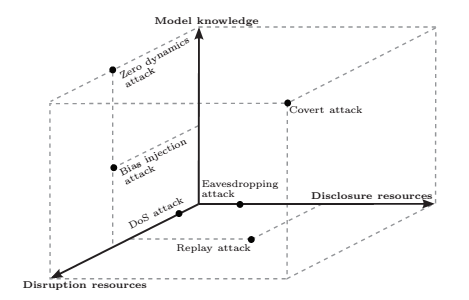
\includegraphics[scale=.4]{fig/attspace.png}\\
	{\scriptsize Source: A. Teixeira, ``Secure Control Systems'' (2014), PhD Thesis}
\end{frame}

\subsection{Countermeasures}

\begin{frame}
	\frametitle{Defence}
	\centering\footnotesize
	\renewcommand{\arraystretch}{1.5}
	\begin{tabular}{l|p{7cm}}
		Class of attack & Defence \\
		\hline
		Disclosure & 
		\renewcommand{\arraystretch}{1.2}
		\begin{tabular}{p{6cm}}			
			\tabitem Sensor placement to exploit geometric conditions \\  \tabitem Differential privacy
		\end{tabular} \\
		\hline 
		Integrity & 
		\renewcommand{\arraystretch}{1.2}
		\begin{tabular}{l}
			\tabitem Signal watermarking \\ 
			\tabitem Moving target, system augmentation \\
			\tabitem Hashing
		\end{tabular} \\
		\hline
		DoS & Resilient design
	\end{tabular}

	\raggedright\vfill
	Caveats:
	\begin{itemize}
		\item Some specific attacks remain to be dealt with
		\item Defence measures introduce control trade-offs.
	\end{itemize}
\end{frame}

\section{Distributed Systems}

\begin{frame}
	\frametitle{A slightly different take on modelling}

	Centralized approaches are resource-heavy and monolithic models are not available.

	\medskip
	We partition a system in $N$ subsystems $\mathcal N_i$:
	\vfill
	\begin{columns}
		\begin{column}{0.5\linewidth}
			\begin{equation*}
				\hspace*{2ex}
				%\mathcal S_i \, : \left\{
				\begin{aligned}
					&x_i(k+1) = A_{i} x_i(k) + B_i \tilde u_i(k) \\
						&\hspace{10ex} + \sum_{j \in \mathcal{N}_i} A_{ij} x_j(k)  + w_i(k)\\
					&y_i(k) = C_i x_i(k) + v_i(k) 
				\end{aligned}\label{eq:CPS-i}
				%\right.
			\end{equation*}
		\end{column}
		\begin{column}{0.49\linewidth}
			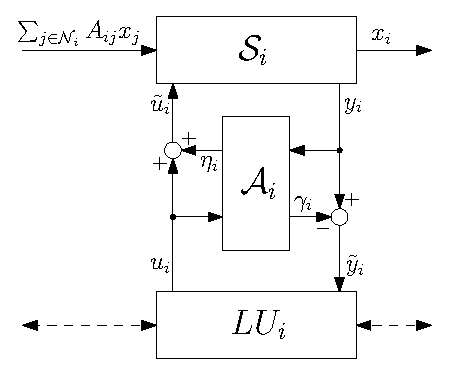
\includegraphics[width=\textwidth]{fig/ndist-obs-generic-ecc.eps}
		\end{column}
	\end{columns}
\end{frame}

\begin{frame}
	\frametitle{Locality}
	\centering
	Stealthiness definitions can adjusted to deal with local subsystems

	\vfill
	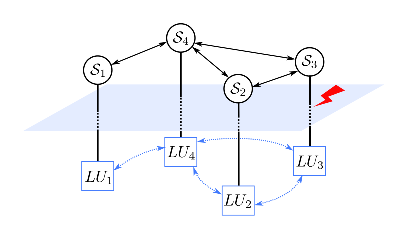
\includegraphics[]{fig/ecc19lss.eps}

	\vfill
	\emph{If control is decoupled} an attack needs to be stealthy only \emph{locally}.
	However, \\[2ex]
	local undetectability $\nRightarrow$ global undetectability
\end{frame}

\begin{frame}
	\frametitle{Basic concept}
	
	\centering
	\begin{block}{}
		Physical interconnections can be leveraged for the purpose of detectability
	\end{block}

	\vfill
	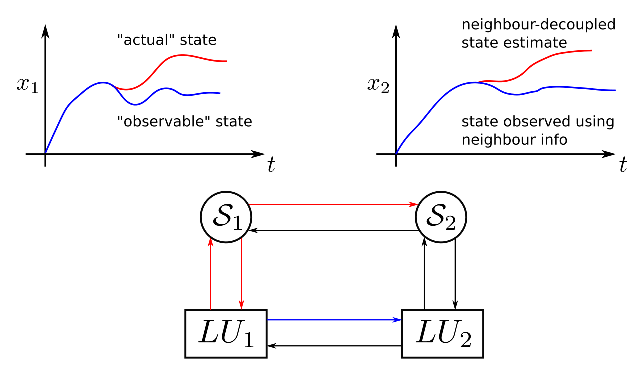
\includegraphics[scale=0.7]{fig/ecc-concept.eps}

	\vfill\footnotesize
	This is a generic concept, independent of how we model $\mathcal S_i$.
\end{frame}

\subsection{Local covert attacks detection}

\begin{frame}
	\frametitle{Local covert attacks}

	\begin{itemize}
		\setlength{\itemsep}{2ex}
		\item<1-> LTI interconnected model with $w_i, v_i$ i.i.d. zero-mean Gaussian with variance $W_i$ and $V_i$.
		
		\item<2-> For a chosen $\eta_i(k)$, the compensation is computed using a replica of the original model $(A_i^a, B_i^a, C_i^a) = (A_i,B_i,C_i)$
		
		\begin{equation*}
			\begin{aligned}
				&x^{a}_i(k+1) = A^a_i x^a_i(k) + B^a_i \eta_i(k) \\
				&\gamma_i(k) = C^a_i x^a_i(k) \,
			\end{aligned}
		\end{equation*}

		\item<3> This attack is \emph{locally stealthy}, as attacked $\tilde y_k$ is undistinguishable from the nominal response.
	\end{itemize}
\end{frame}

\begin{frame}
	\frametitle{Unbiased minimum-variance estimation}
	Design a filter with gains $M_i(k)$ and $\bar L_i(k)$
	\begin{align*}
		&\hat{x}_i(k) =  (I - \bar L_i(k)C_i)\left[A_i\hat{x}_i(k-1) + B_i u_i(k-1)\right] +\bar L_i(k) \tilde y_i(k) \\
		&\hat{\xi}_i(k-1|k) = M_i(k)\left[\tilde{y}_i(k) - C_i \left(A_i\hat{x}_i(k-1) + B_i u_i(k-1)	\right) \right]
	\end{align*}
	
	\vfill
	Only the independent components of the interconnections can be estimated
	$$
		\sum_{j\in\mathcal{N}_i}A_{ij} x_j = \row{j\in\NN_i}\left[A_{ij}\right]\col{j\in\NN_i}\left[x_i\right] = G_i \bar{E}_i \zeta_i = G_i \xi_i
	$$
	with $G_i$ full rank.
\end{frame}

\begin{frame}
	\frametitle{Residual design}
	The residual
	$$
	\hat \rho_i(k-1|k) \doteq  \hat \xi_i(k-1|k) - \bar{E}_i \col{j\in\NN_i}[\hat x_j(k-1)]
	$$
	contains information about the discrepancy: \\[3ex]
	\centering

	\noindent{\color{blue}\fbox{
		\normalcolor\parbox{15em}{
			\centering 
			Communicated $\hat x_j$ \\
			(containing possible false data)
		}
	}} \\[2ex]
	vs \\[2ex]
	\noindent{\color{red}\fbox{
		\normalcolor\parbox{15em}{
			\centering 
			Estimated $\hat\xi_i$ \\ 
			(explaining the current estimate)
		}
	}}
\end{frame}

\begin{frame}
	\frametitle{Detection strategy}

	For a deterministic attacker in $\mathcal S_j$, $$\mean{\hat \rho_i(k-1|k)} \propto x_j^a(k-1), $$ and since impact $\propto x_j^a$, we can detect an attack via GLR test on a sliding window of $\hat \rho_i$.

	$$
	\sum_{\kappa = k-\omega+1}^{k} 
	\underbrace{\hat \rho_i(\kappa-1|\kappa)^\top U_i(\kappa)^\top}_{\hat z_i(k)^\top} 
	\underbrace{\Lambda_i(\kappa)^{-1}}_{\text{diagonal}} 
	\underbrace{U_i(\kappa)\hat \rho_i(\kappa-1|\kappa)}_{\hat z_i(k)} > \theta_i(k)
	$$

	For each component, test confidence against $\chi^2_\omega(0)$.
\end{frame}

\begin{frame}
	\frametitle{Example -- Spring-connected pendula}
	\begin{equation*}
		m_il_i^2\Ddot{\delta}_i = m_igl_i\delta_i + u_i + \sum_{j\in\NN_i} k_{ij}a_i^2(\delta_j-\delta_i)
	\end{equation*}
	\centering
	Discretize each subsystem using Euler's approximation.
	
	\vfill
	\begin{columns}
		\begin{column}{0.75\linewidth}
			Attack $\mathcal S_3 $ at $k_a = 35$ s
			$$\eta_3(k) \doteq 0.5 \left(1-e^{-0.3 (k\cdot T_s-k_a)}\right)\,\mathrm{sin}\left(\frac{2}{30} \pi k \cdot T_s\right)$$

			Compensation $\gamma_3$ obtained with exact subsystem model.
		\end{column}
		\begin{column}{0.23\linewidth}
			%\raggedleft
			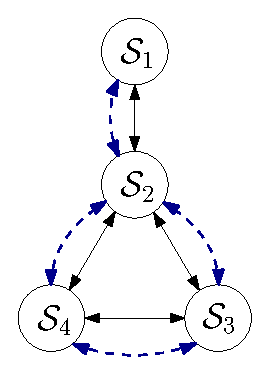
\includegraphics[scale=0.6]{fig/layout.eps}
		\end{column}
	\end{columns}
\end{frame}

\begin{frame}
	\frametitle{Example -- Simulation results}
	\vspace{2ex}
	\centering
	\begin{tabular}{lr}
		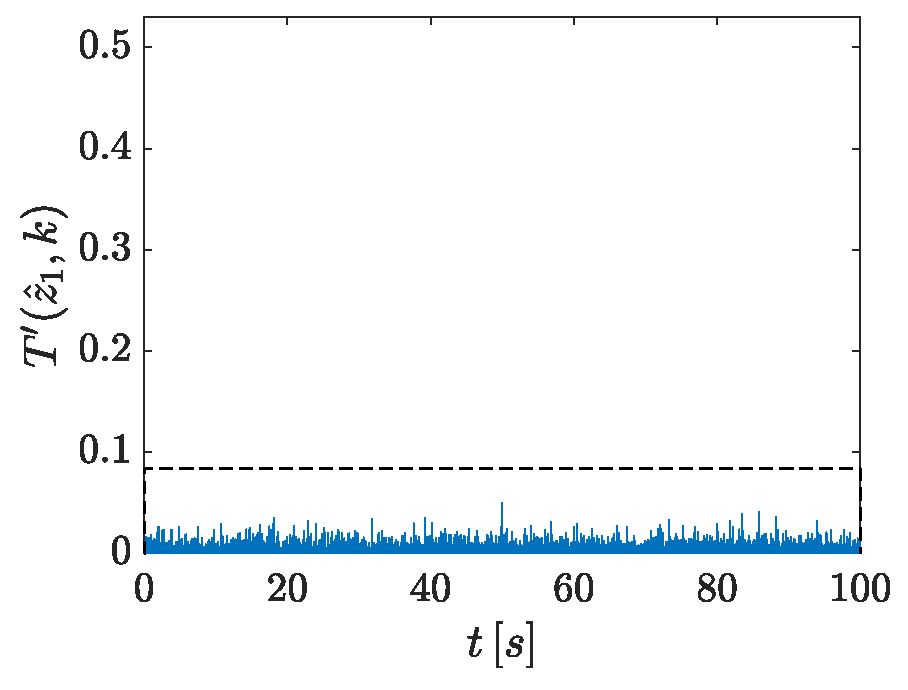
\includegraphics[width=0.4\linewidth]{fig/det1_okThr.eps} & 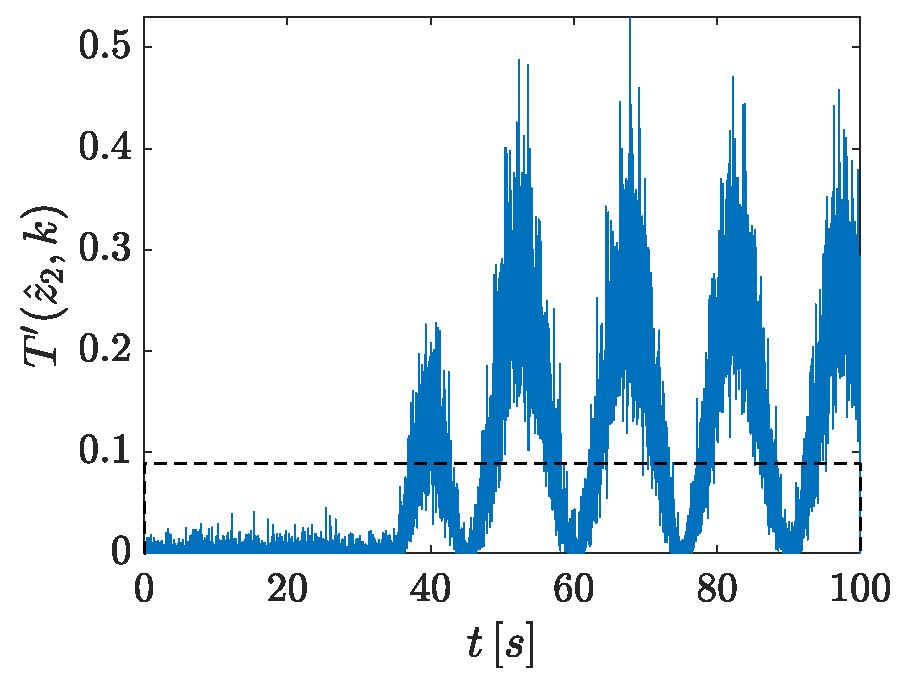
\includegraphics[width=0.4\linewidth]{fig/det2_okThr.eps} \\
		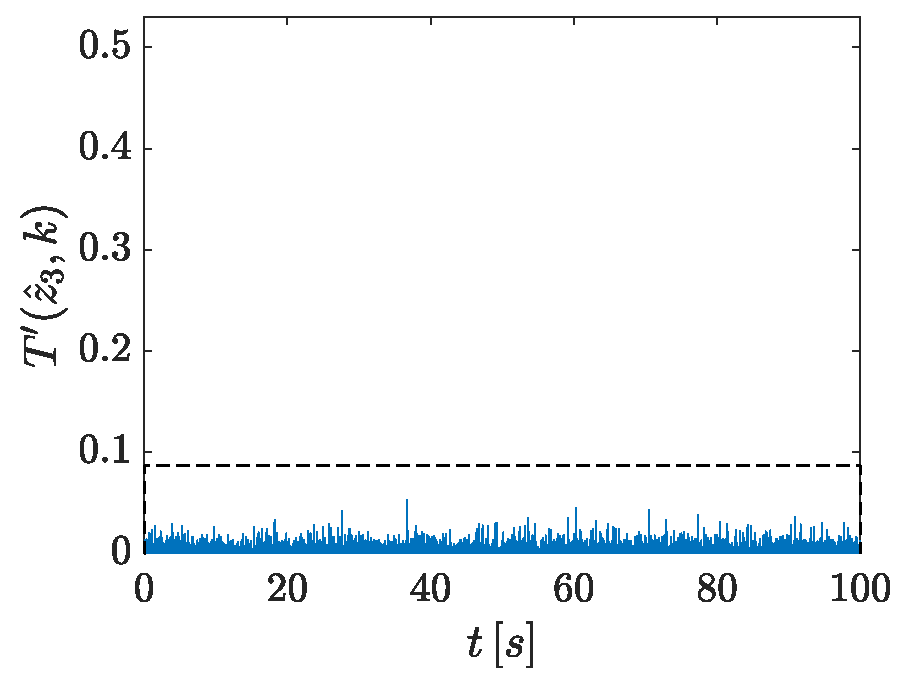
\includegraphics[width=0.4\linewidth]{fig/det3_okThr.eps} & 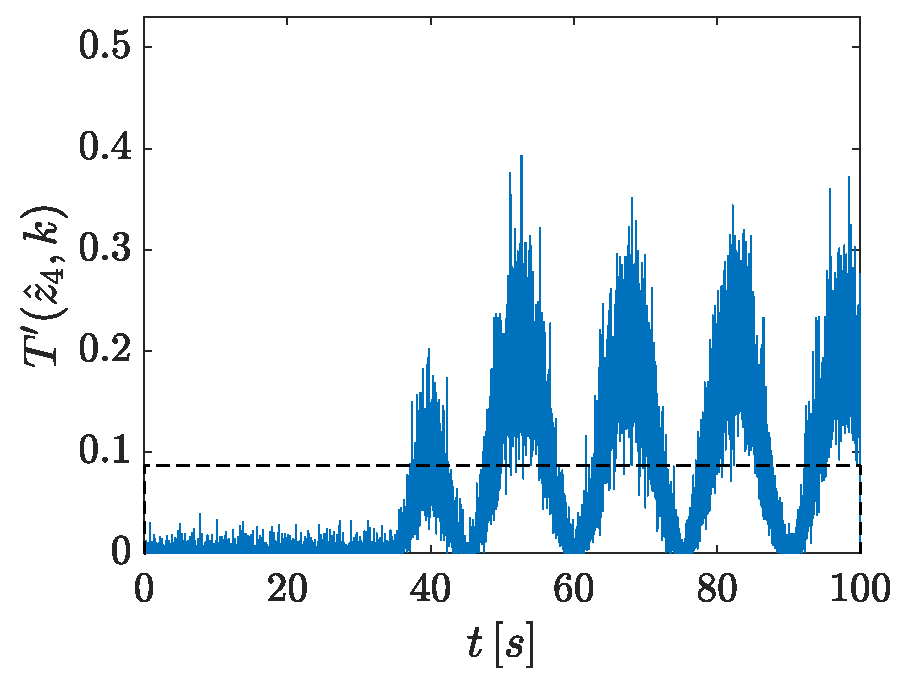
\includegraphics[width=0.4\linewidth]{fig/det4_okThr.eps}
	\end{tabular}	
\end{frame}

\section{What's next?}

% \begin{frame}
% 	\frametitle{Limitations}

% \end{frame}

\begin{frame}
	\frametitle{Future work}
	\begin{itemize}
		\setlength{\itemsep}{1.5ex}
		\item<1-> Structural/geometric/topological characterization of attack detectability in interconnected systems
		
		\item<2-> Relaxing attacker knowledge for covert attacks, i.e. the plant's model is known with some bounded uncertainty
		
		\item<3> The residual represents the error of the input estimate of a neighbour.
		
		Can we correct $\hat x_i + \delta$ such that $u_j(x_i + \delta)$ compensates the attack?
	\end{itemize}
\end{frame}

\begin{frame}
	\frametitle{Gaps}	
	\begin{itemize}
		\setlength{\itemsep}{1.5ex}
		\item<1-> More attention to the \emph{confidentiality} part of the problem, with signal or system based techniques to enforce authenticity and keep secrecy
		
		\item<2-> Game theoretic approaches in a distributed setting have just started to be taken into consideration
	
		\item<3-> Attack-tolerant control: detect, isolate, compensate, (reconfigure) to guarantee certain operating performance (cf. FTC)
		
		\item<4-> More general class of systems (switching, event-driven, etc.) but also attacks tailored on specific sensitive systems
		
		\item<5> Non-model-based approaches. 
	\end{itemize}
\end{frame}
 
\begin{frame}
	\frametitle{Some notable references}
	\nocite{*}
	\printbibliography
\end{frame}

\end{document}